\chapter{Einleitung}
Im Projekt Med-Eval ist eine Web-Applikation für die Unterstützung
von klinischen Studien entstehen. 
Studienteilnehmer/innen sollen per QR-Code den Link zum Studien-
Fragebogen öffnen. Die Navigation durch den Fragebogen soll auf dem Endgerät
(Laptop/Smartphone) schrittweise erfolgen, und lokal überprüft sein.
Die Daten kann jederzeit vom Server abgerufen werden, für eine später Auswertung.
Wir nutzen hierfür das Open Source Tool Limesurvey, welches wir für die
medizinische Umgebung angepasst haben.
Die Verbindung bei einer Umfrage und Abruf der Daten werden über SSL gesichert werden.
Auch der Server ist gegen die gängigsten Angriffsarten abgesichert.
Die Software kann durch das Ansible Deployment System auf jeden beliebigen Server, welcher die Voraussetzungen erfüllt,
innerhalb von kurzer Zeit installiert werden.
Limesurvey ist ein modulares Baukasten-System für die Erstellung der Fragebögen konfigurierbar.
Wir haben es um einen weitere Fragetyp, welche es einem Teilnehmer einer Umfrage ermöglicht
ein oder mehrere Körperteile anzugeben.
Des weiteren haben wir eine Möglichkeit erarbeitet einer Umfrage Umweltdaten wie Wetter und Mondstand
hinzufügen basierend auf dem Standort des Umfrageteilnehmers. Dies Daten können im Zusammenhang mit der Wirksamkeit eines
Medikaments eine Rolle spielen.
Die Umfrage sollte auf Desktop sowie gängigen Smartphone nutzbar sein.

\begin{figure}[!ht]
\centering
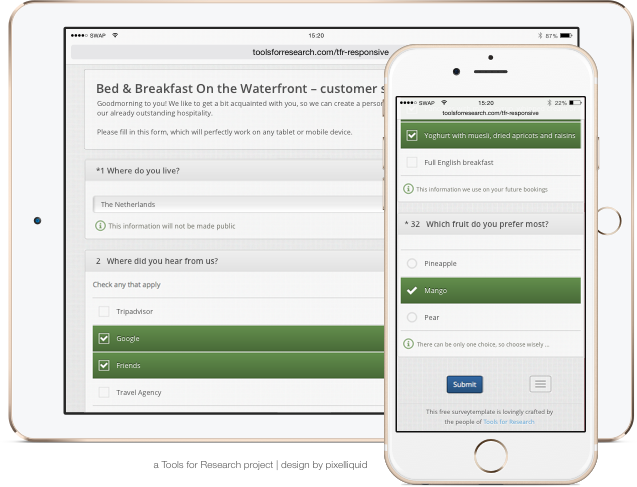
\includegraphics[width=0.6\textwidth]{content/pictures/preview.png}
\caption{Beispiel Desktop and Mobile Umfrage}
\url{https://www.toolsforresearch.com/sites/toolsforresearch.com/files/preview.png}
\label{fig_holo3}
\end{figure}


